
\subsection{ AI4Test }\

AI4Test project main \textbf{objectives}: (2024.1.1-2024.12.1)

\begin{itemize}
    \item Optimize Test Book Generation: Automatically Support the Test Engineering Team in designing the Test Books;
    \item Standardize Test Cases: Normalize Test Cases through a unified Common Test Case Language Model;
    \item Transform Unstructured Test Cases with AI: Utilize AI models to convert unstructured Test Cases into a standardized Common Language Model;
    \item AI-Driven Requirements-to-Test Cases Modeling: Create an AI model for predicting and automating test generation, prioritization, reporting test durations, and forecasting failure probabilities based on product requirements;
    \item New Test Cases Scenarios: Explore the generation of novel Test Cases from product requirements using large language models (LLMs).
\end{itemize}

How to start and use AI4Test ?

\vspace{0.5cm}

\begin{lstlisting}
# create and use python virtual enviroment
conda activate ai4test

# Start AI4Test Webserver
cd /data/git/ai4test
python3 Infrastructure/app/main.py

# WebSite address
http://172.16.33.244:8882/
\end{lstlisting}

1/ The main user interface for AI4Test 

\begin{figure}[H]
    \begin{center}
        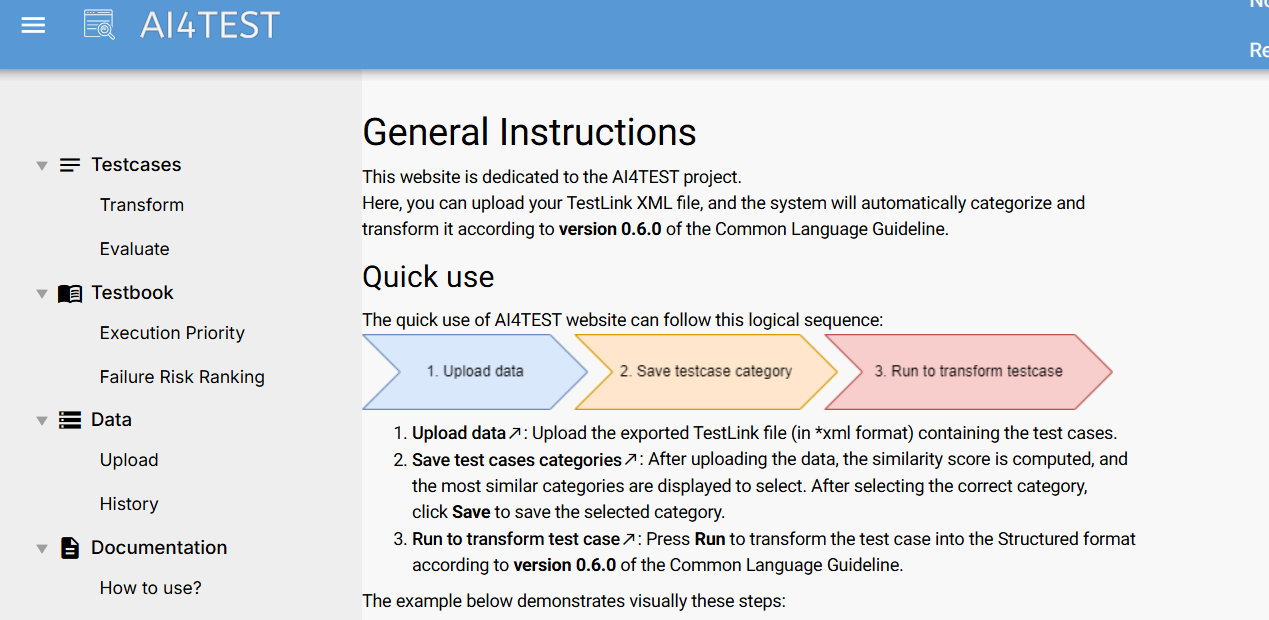
\includegraphics[width=.95\linewidth]{res/ai4test-main.png}\\
        \caption{AI4Test main UI}\label{ai4test-main}
    \end{center}
\end{figure}

/2  When using the tool for the first time, you need to upload test cases in XML format, which can be directly exported from TestLink. In addition, you can upload requirement documents—docx or xls files are supported.

\begin{figure}[H]
    \begin{center}
        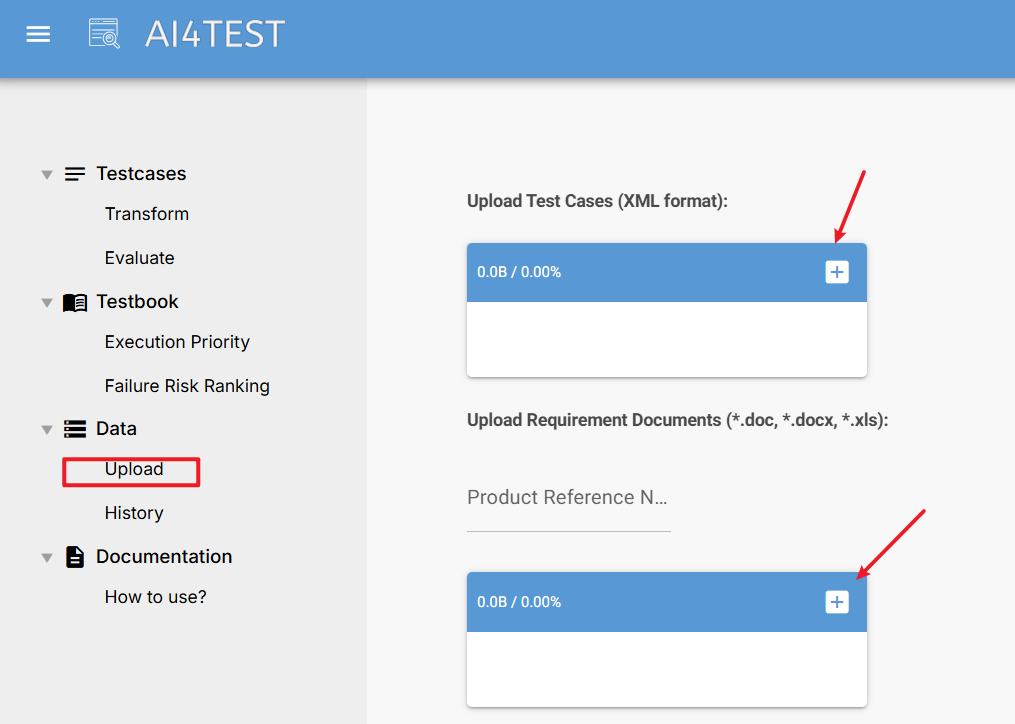
\includegraphics[width=.95\linewidth]{res/ai4test-uploa.png}\\
        \caption{Upload files to AI4Test}\label{ai4test-uploa}
    \end{center}
\end{figure}

3/  Loading requirements and test cases can be done by selecting them from the history of uploaded data

\begin{figure}[H]
    \begin{center}
        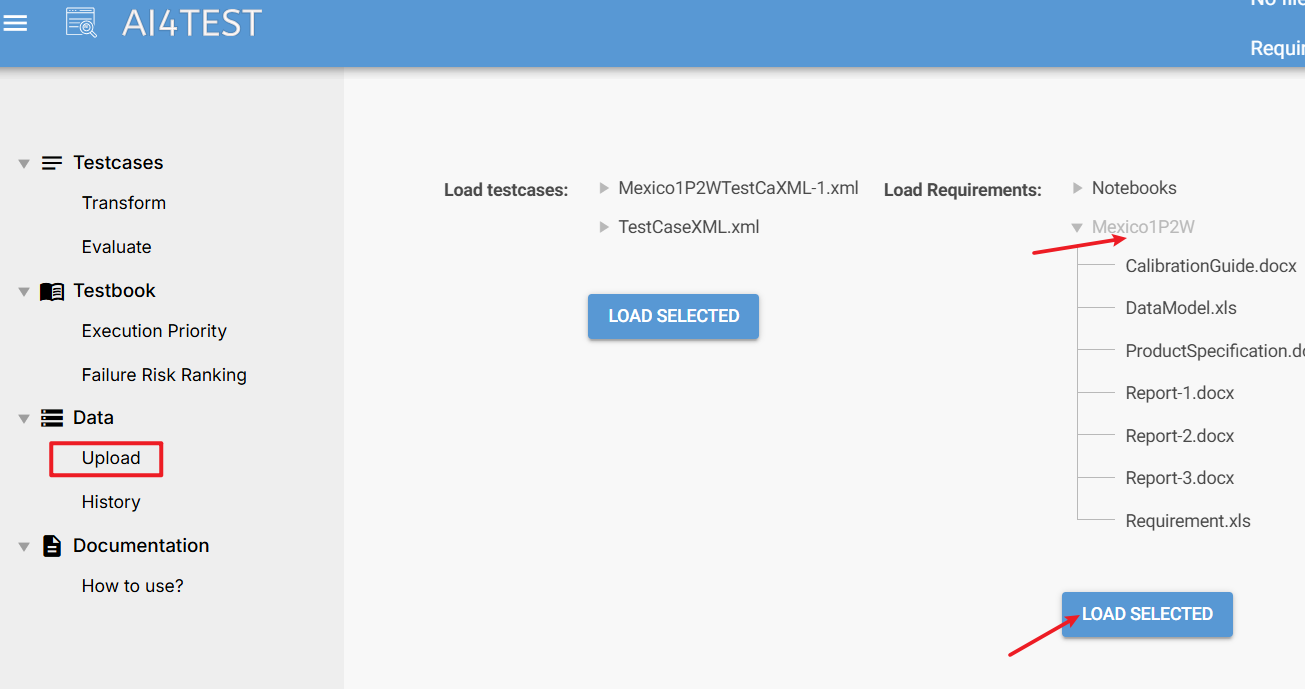
\includegraphics[width=.95\linewidth]{res/ai4test-history1.png}\\
        \caption{Loading requirements}\label{ai4test-history1}
    \end{center}
\end{figure}

\begin{figure}[H]
    \begin{center}
        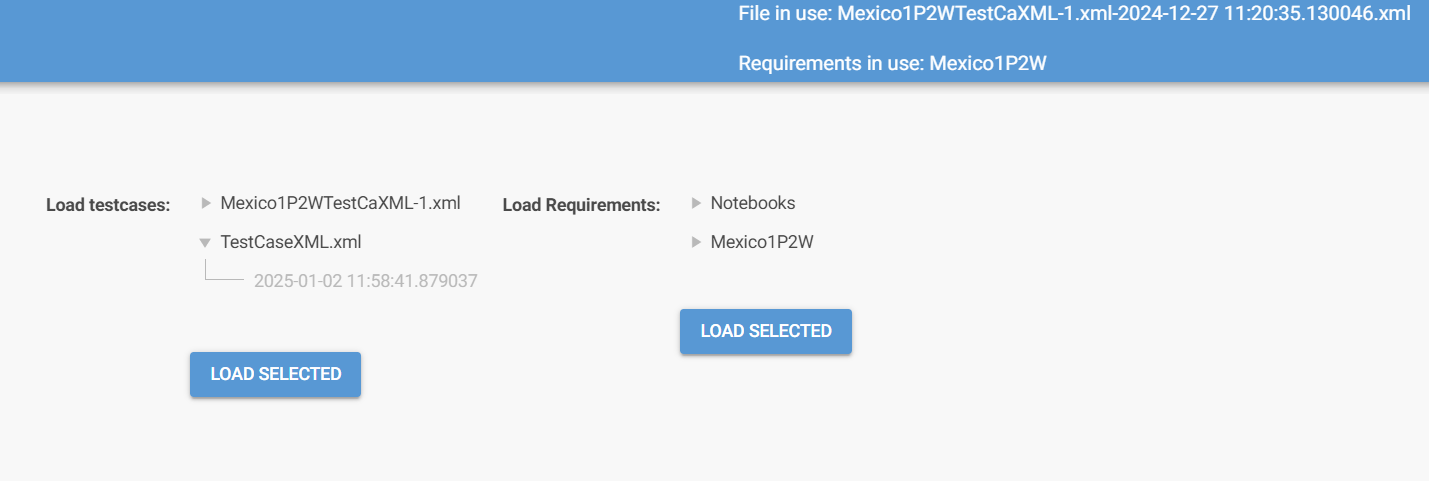
\includegraphics[width=.95\linewidth]{res/ai4test-history2.png}\\
        \caption{Loading test cases}\label{ai4test-history2}
    \end{center}
\end{figure}

4/  From the Transform section of the Testcases page in the left‑hand tree, you can view the AI conversion results, whereby test cases exported from TestLink are transformed into structured test cases defined by the Common Test Language specification

\begin{figure}[H]
    \begin{center}
        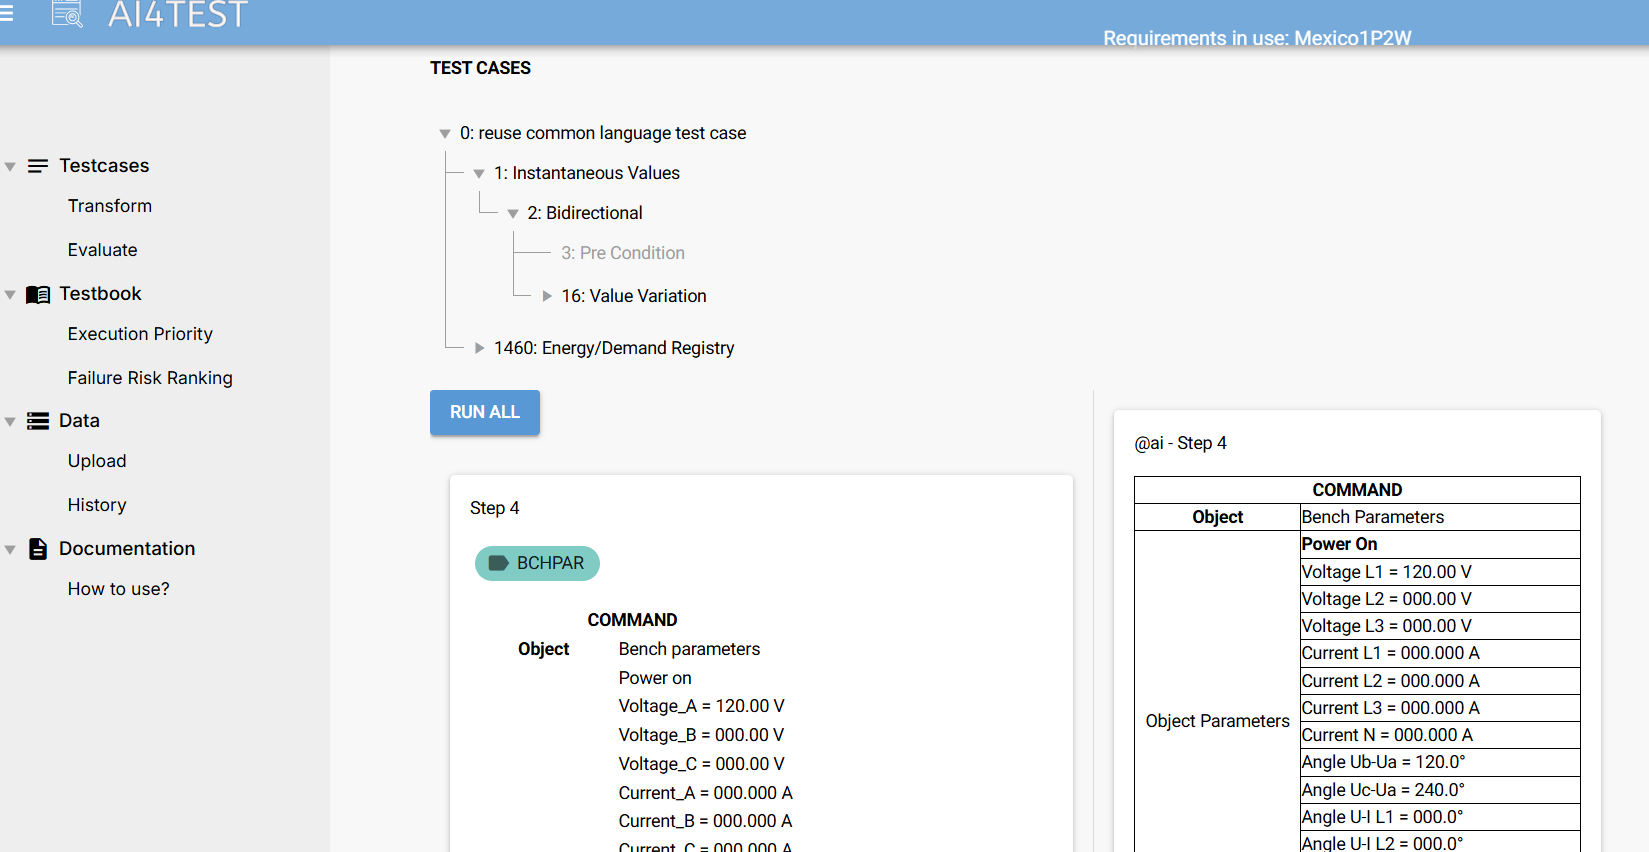
\includegraphics[width=.95\linewidth]{res/ai4test-transformcase.png}\\
        \caption{Test Case transformation }\label{ai4test-transformcase}
    \end{center}
\end{figure}

5/  If the AI‑converted result is incorrect, you can manually correct it.
You can select a different classification, and other categories are also available in the Additional section. Once you submit your feedback, the system will automatically retrain and learn from it.

\begin{figure}[H]
    \begin{center}
        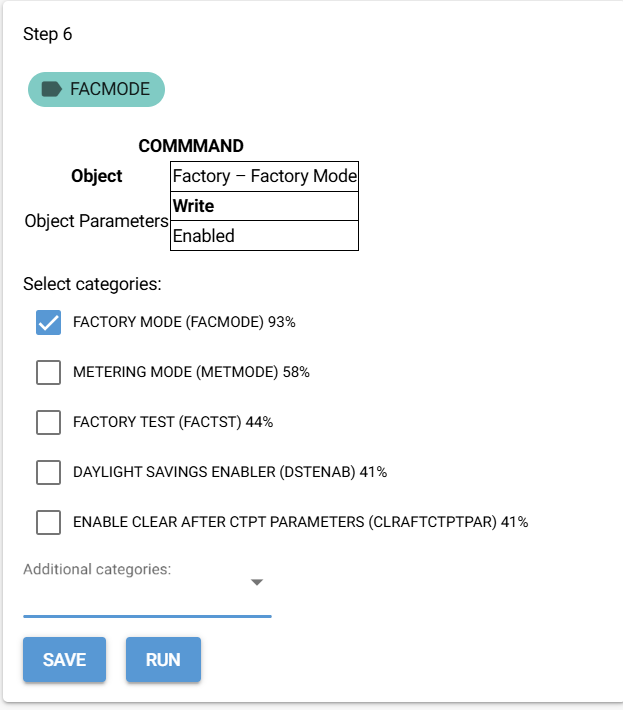
\includegraphics[width=.95\linewidth]{res/ai4test-manual.png}\\
        \caption{Manual adjustment of conversion results }\label{ai4test-manual}
    \end{center}
\end{figure}

6/  Each category is accompanied by a probability—the higher the value, the stronger the AI’s recommendation.

\begin{figure}[H]
    \begin{center}
        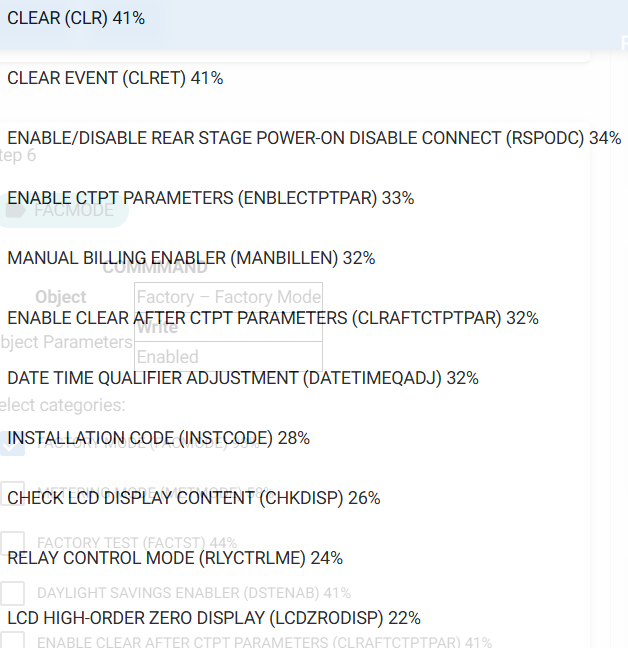
\includegraphics[width=.95\linewidth]{res/ai4test-category.png}\\
        \caption{Execution step classification}\label{ai4test-category}
    \end{center}
\end{figure}

7/  Sort the test cases by execution success rate based on their historical execution results.

\begin{figure}[H]
    \begin{center}
        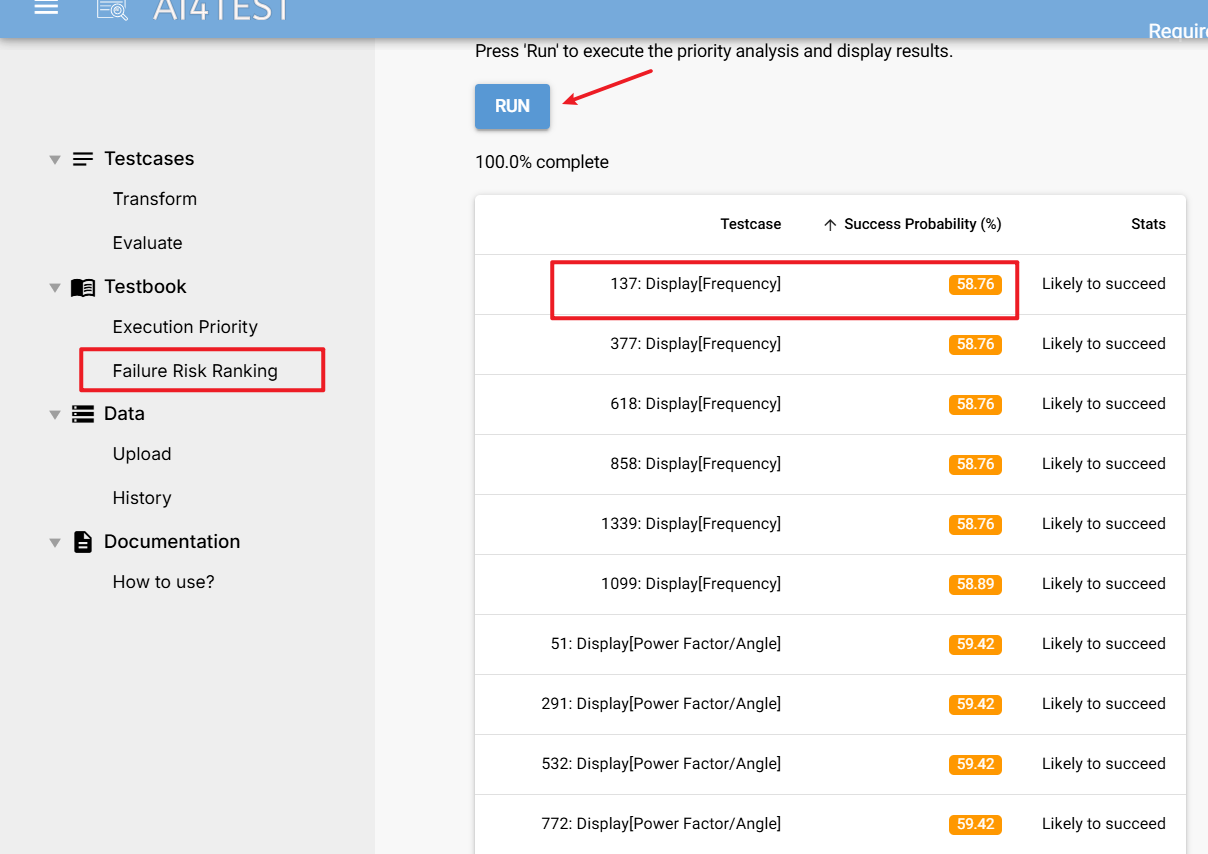
\includegraphics[width=.95\linewidth]{res/ai4test-priority.png}\\
        \caption{Test case execution success rate }\label{ai4test-priority}
    \end{center}
\end{figure}

\section{Closing remarks}\

All of the contents in this document represnets my exploration in AI while learning, supplemented by references to various project documents. There may be some errors and omissions, so please feel free to contact me if you find any. I would also like to thank the members of the AI4Test team — \textbf{Francisco Alexandre} and \textbf{Wang Wen}—as well as\textbf{ Gabriel} from the OCR project. Though I was involved in both projects from start to finish, I appreciate their contributions.